% =====================================================================
% 4. Area 1 in code: Dense and CNN (own), RNN and Transformer (MM, summary)
% =====================================================================
\section{Area 1: core architectures in PyTorch}\label{sec:arch-code}

Each block has a model file in \texttt{src/models/}, registered by name so that
\texttt{python -m src.train --model <name>} can build it, an experiment script
(\texttt{src/<block>\_experiments.py} with \texttt{run}, \texttt{final} and \texttt{report}) and a test
file. The theory and the analysis of the results are in the PRDL-DL report; this section is about the
implementation and the training behaviour.

\subsection{Dense network (own block)}

\lstinputlisting[firstnumber=34,caption={Hidden blocks of \texttt{DenseNet} (\texttt{src/models/dense.py},
lines 34--51).},label={lst:dense}]{common/code/dense_net.py}

\begin{itemize}[leftmargin=1.2em,itemsep=1pt]
  \item \textbf{Flatten order.} \texttt{nn.Flatten} on $(B, 12, 1000)$ puts the 1000 samples of lead I
        first, then lead II, etc.; reshaping the first-layer weight to (units, 12, 1000) gives back one
        pattern per lead, which is how Figure~\ref{fig:dense_first_layer} was drawn.
  \item \textbf{The training loss is measured in training mode}, with dropout active, so it is higher
        than the loss of the same weights in evaluation mode; this is why in the first epochs the
        training curve can lie above the validation curve (Figure~\ref{fig:dense_curves}).
  \item \textbf{Batch norm in evaluation} uses running averages collected in training; forgetting
        \texttt{model.eval()} would make a prediction depend on the other records of the batch.
        \texttt{BatchNorm1d} also refuses a training batch of one record, a case we checked could not
        occur with our split sizes.
  \item \textbf{Cost.} One epoch takes \denseEpochTimeMeanBase{}\,s for the baseline; the network has
        \denseParamsBase{} parameters, almost all in the first Linear layer.
\end{itemize}

% Shared float (common/make_floats.py). Figure: figures/dense_curves.pdf
\begin{figure}[htbp]
\centering
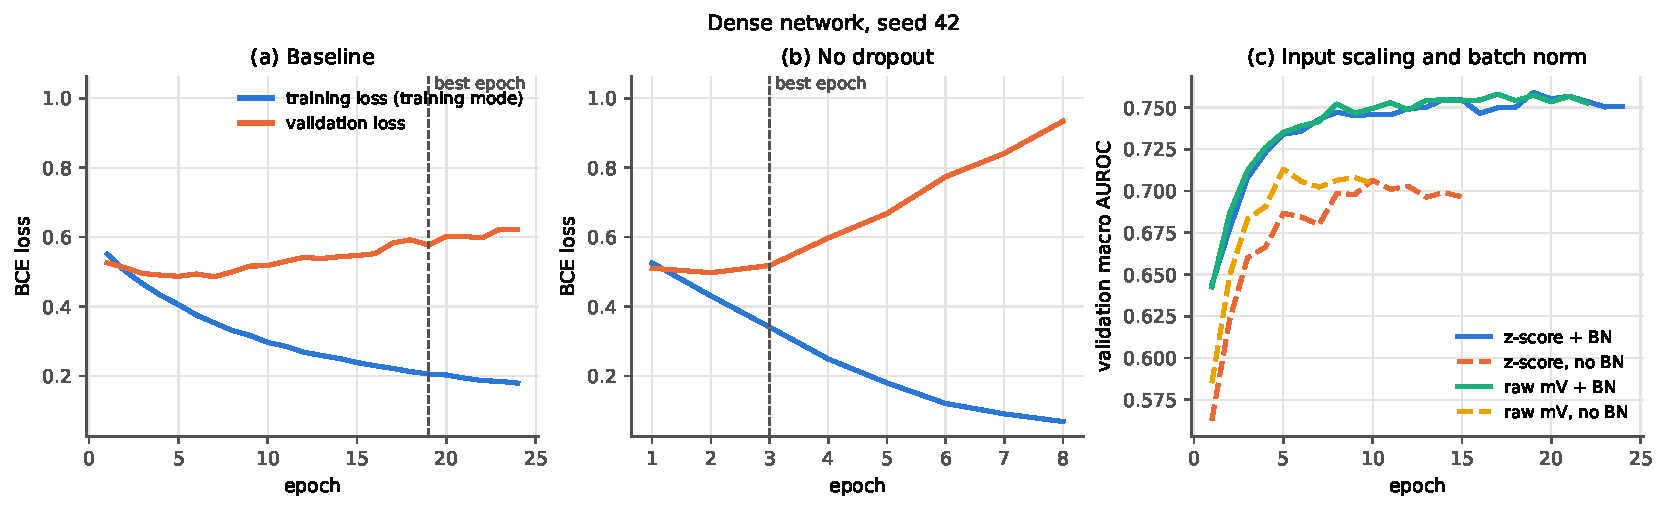
\includegraphics[width=\textwidth,height=0.42\textheight,keepaspectratio]{figures/dense_curves.pdf}
\caption[Dense network: learning curves]{Dense network, seed 42. (a) Baseline: training loss (measured in training mode, with dropout) and validation loss; dashed line: best epoch by validation macro AUROC. (b) The same without dropout. (c) Validation macro AUROC with and without input z-score and batch norm.}
\label{fig:dense_curves}
\end{figure}

% Shared float (common/make_floats.py). Figure: figures/dense_first_layer.pdf
\begin{figure}[htbp]
\centering
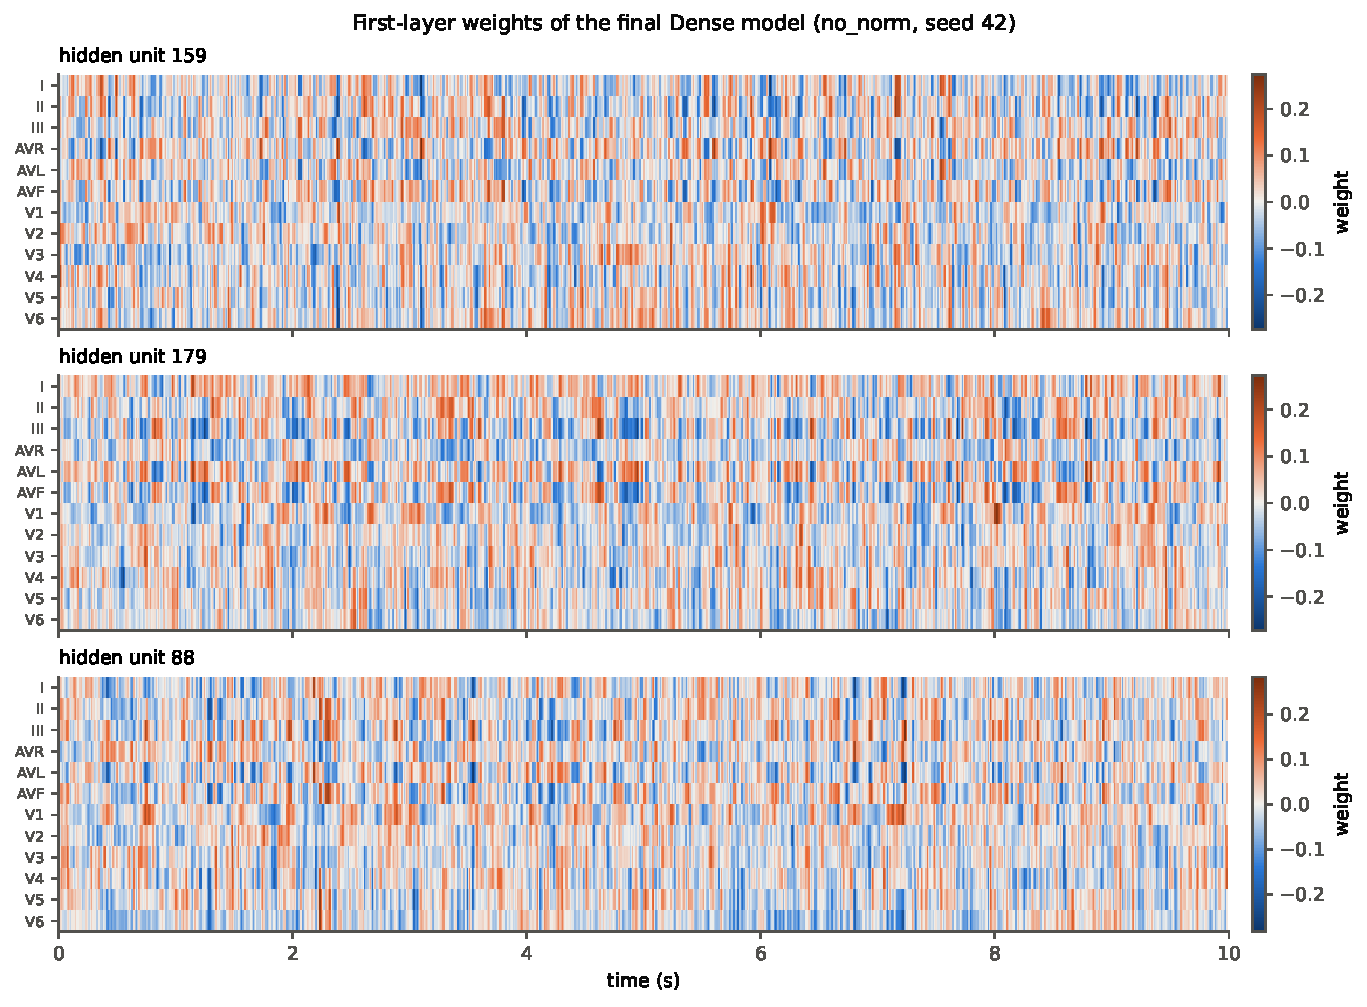
\includegraphics[width=\textwidth,height=0.42\textheight,keepaspectratio]{figures/dense_first_layer.pdf}
\caption[Dense network: first-layer weights]{First-layer weights of the final Dense model (\texttt{no\_norm}, seed 42) for the three hidden units with the largest weight norm, reshaped to 12 leads $\times$ 1000 samples.}
\label{fig:dense_first_layer}
\end{figure}


\subsection{1D CNN (own block)}

\lstinputlisting[firstnumber=31,caption={Residual block of the CNN (\texttt{src/models/cnn.py}, lines
31--70).},label={lst:conv}]{common/code/conv_block.py}

\begin{itemize}[leftmargin=1.2em,itemsep=1pt]
  \item \textbf{Layout.} \texttt{Conv1d} expects $(B, \text{channels}, \text{time})$; the cache already
        stores $(12, 1000)$, so no \texttt{permute} is needed. A $(B, \text{time}, \text{channels})$
        tensor would silently treat the 1000 samples as channels.
  \item \textbf{``Same'' padding needs an odd kernel.} \texttt{padding = k // 2} keeps the length only
        for odd $k$; the model refuses even kernels because the main path and the shortcut must have the
        same length to be added.
  \item \textbf{The skip connection is a plain \texttt{+}} (line 69). The identity shortcut adds no
        parameter, a $1\times1$ convolution adapts the number of channels where it changes, and autograd
        sends the gradient through both branches.
  \item \textbf{Receptive field.} \texttt{CNN1D.receptive\_field()} computes it from kernels and pooling;
        a test checks it against the gradient of a linearised copy of the network.
  \item \textbf{Interpretation.} Feature maps are read with forward hooks
        (\texttt{register\_forward\_hook}), removed in a \texttt{finally} block. With global average
        pooling and one Linear layer, the logit equals the bias plus the mean over time of the class
        activation map, in evaluation mode (in training mode dropout breaks the identity); a test checks
        it numerically.
  \item \textbf{Cost.} \cnnEpochTimeMeanBase{}\,s per epoch for the baseline, against
        \denseEpochTimeMeanBase{}\,s for the Dense network, with \cnnParamsBase{} parameters.
\end{itemize}

% Shared float (common/make_floats.py). Figure: figures/cnn_curves.pdf
\begin{figure}[htbp]
\centering
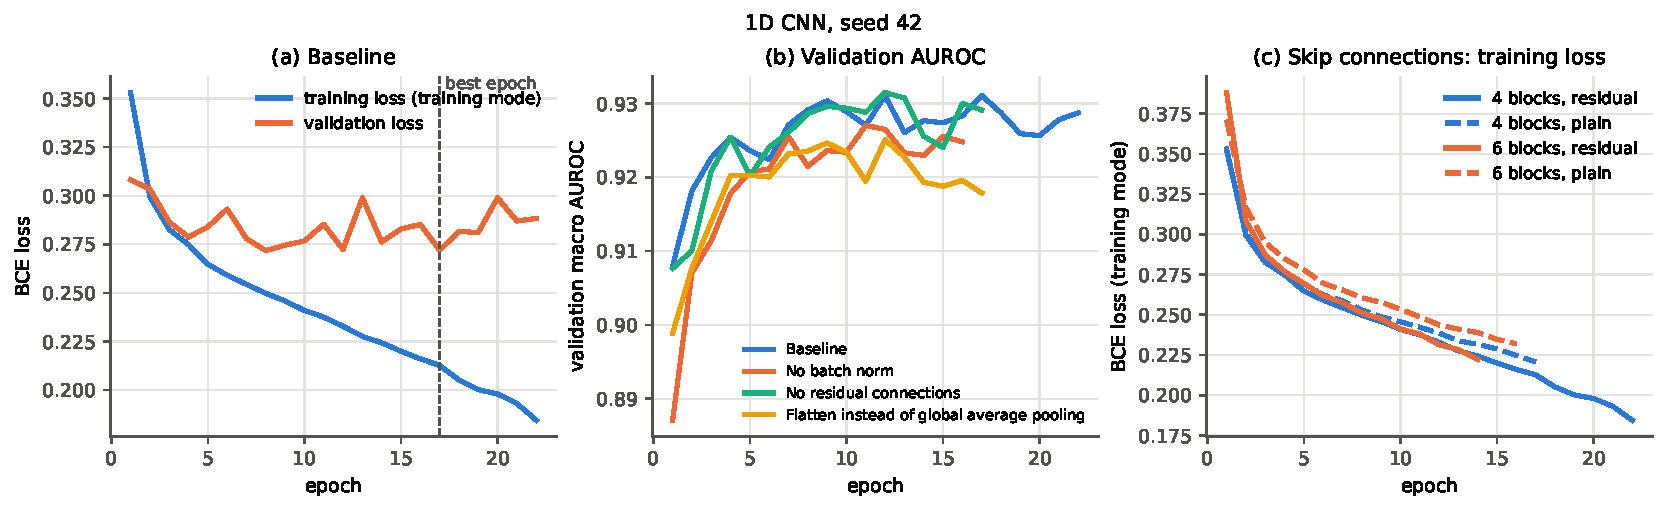
\includegraphics[width=\textwidth,height=0.42\textheight,keepaspectratio]{figures/cnn_curves.pdf}
\caption[1D CNN: learning curves]{1D CNN, seed 42. (a) Baseline training and validation loss; dashed line: best epoch. (b) Validation macro AUROC without batch norm, without residual connections and with flatten instead of global average pooling. (c) Training loss with and without residual connections, at 4 and 6 blocks.}
\label{fig:cnn_curves}
\end{figure}


\subsection{Recurrent networks and Transformer (Mar\'ia's blocks, summary)}

\begin{itemize}[leftmargin=1.2em,itemsep=1pt]
  \item \textbf{Sequence layout.} The record $(B, 12, 1000)$ becomes a sequence $(B, T, \text{features})$
        with \texttt{batch\_first=True}, the opposite axis order of \texttt{Conv1d}: 100 frames of
        10 samples (120 numbers per step), 1000 raw steps, or the 125 steps of a convolutional front end
        that reuses the CNN's \texttt{ConvBlock}.
  \item \textbf{Readouts.} The last state is \texttt{h\_n[-1]} (last layer); mean pooling averages
        \texttt{out} over time; attention pooling scores each state, applies a softmax over time and
        takes the weighted sum.
  \item \textbf{Stability and determinism.} Gradient clipping at norm 1 in every configuration, and
        \texttt{CUBLAS\_WORKSPACE\_CONFIG} so that the GPU runs of \texttt{nn.LSTM} are reproducible.
  \item \textbf{Hand-written attention.} \texttt{src/models/attention.py} implements scaled dot-product
        attention, multi-head attention and a Pre-LN/Post-LN Transformer block as in the course
        notebooks, with an optional causal mask (Listing~\ref{lst:causal}); a test checks it against
        \texttt{nn.MultiheadAttention} with the same weights, with and without the mask. Patches are
        embedded by a Linear layer, which a test shows to be a \texttt{Conv1d} with kernel and stride 10.
  \item \textbf{Cost.} The 1000-step LSTM is the slowest classifier (\rnnEpochTimeMeanRaw{}\,s per
        epoch against \rnnEpochTimeMeanBase{}\,s with 100 frames) and needs many more epochs, the
        difficulty of backpropagation through many time steps; the Transformer baseline takes
        \transformerEpochTimeMeanBase{}\,s.
\end{itemize}

% Shared float (common/make_floats.py). Figure: figures/rnn_curves.pdf
\begin{figure}[htbp]
\centering
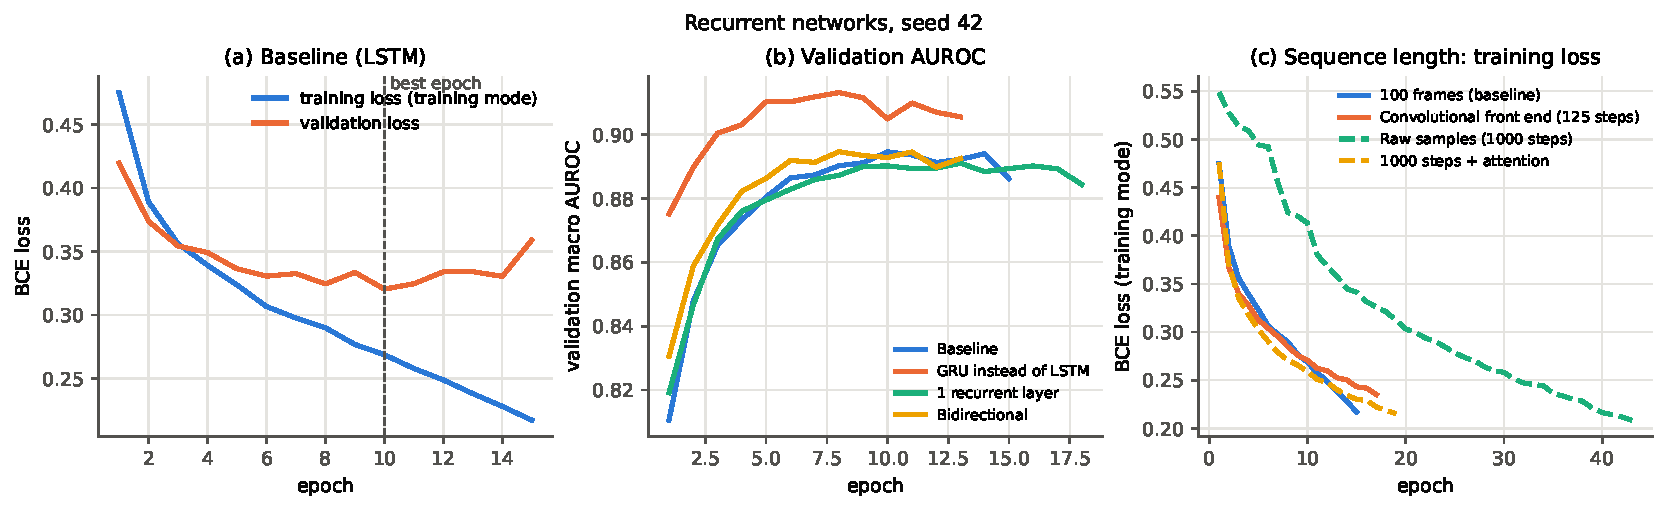
\includegraphics[width=\textwidth,height=0.42\textheight,keepaspectratio]{figures/rnn_curves.pdf}
\caption[Recurrent networks: learning curves]{Recurrent networks, seed 42. (a) LSTM baseline losses. (b) Validation macro AUROC of the baseline, GRU, one recurrent layer and bidirectional LSTM. (c) Training loss with 100 frames, the convolutional front end, 1000 raw steps and 1000 steps with attention.}
\label{fig:rnn_curves}
\end{figure}


Test results of every family are in Table~\ref{tab:comparison_final} (Section~\ref{sec:code}).
In the Dense and CNN blocks the validation loss reaches its minimum earlier than the validation AUROC,
so early stopping on the AUROC lets the models train past the loss minimum: the ranking of the records
keeps improving while the probabilities become over-confident.
